% Options for packages loaded elsewhere
\PassOptionsToPackage{unicode}{hyperref}
\PassOptionsToPackage{hyphens}{url}
%
\documentclass[
]{book}
\usepackage{lmodern}
\usepackage{amssymb,amsmath}
\usepackage{ifxetex,ifluatex}
\ifnum 0\ifxetex 1\fi\ifluatex 1\fi=0 % if pdftex
  \usepackage[T1]{fontenc}
  \usepackage[utf8]{inputenc}
  \usepackage{textcomp} % provide euro and other symbols
\else % if luatex or xetex
  \usepackage{unicode-math}
  \defaultfontfeatures{Scale=MatchLowercase}
  \defaultfontfeatures[\rmfamily]{Ligatures=TeX,Scale=1}
\fi
% Use upquote if available, for straight quotes in verbatim environments
\IfFileExists{upquote.sty}{\usepackage{upquote}}{}
\IfFileExists{microtype.sty}{% use microtype if available
  \usepackage[]{microtype}
  \UseMicrotypeSet[protrusion]{basicmath} % disable protrusion for tt fonts
}{}
\makeatletter
\@ifundefined{KOMAClassName}{% if non-KOMA class
  \IfFileExists{parskip.sty}{%
    \usepackage{parskip}
  }{% else
    \setlength{\parindent}{0pt}
    \setlength{\parskip}{6pt plus 2pt minus 1pt}}
}{% if KOMA class
  \KOMAoptions{parskip=half}}
\makeatother
\usepackage{xcolor}
\IfFileExists{xurl.sty}{\usepackage{xurl}}{} % add URL line breaks if available
\IfFileExists{bookmark.sty}{\usepackage{bookmark}}{\usepackage{hyperref}}
\hypersetup{
  pdftitle={Falco Tutorial},
  pdfauthor={Ho Lab},
  hidelinks,
  pdfcreator={LaTeX via pandoc}}
\urlstyle{same} % disable monospaced font for URLs
\usepackage{longtable,booktabs}
% Correct order of tables after \paragraph or \subparagraph
\usepackage{etoolbox}
\makeatletter
\patchcmd\longtable{\par}{\if@noskipsec\mbox{}\fi\par}{}{}
\makeatother
% Allow footnotes in longtable head/foot
\IfFileExists{footnotehyper.sty}{\usepackage{footnotehyper}}{\usepackage{footnote}}
\makesavenoteenv{longtable}
\usepackage{graphicx,grffile}
\makeatletter
\def\maxwidth{\ifdim\Gin@nat@width>\linewidth\linewidth\else\Gin@nat@width\fi}
\def\maxheight{\ifdim\Gin@nat@height>\textheight\textheight\else\Gin@nat@height\fi}
\makeatother
% Scale images if necessary, so that they will not overflow the page
% margins by default, and it is still possible to overwrite the defaults
% using explicit options in \includegraphics[width, height, ...]{}
\setkeys{Gin}{width=\maxwidth,height=\maxheight,keepaspectratio}
% Set default figure placement to htbp
\makeatletter
\def\fps@figure{htbp}
\makeatother
\setlength{\emergencystretch}{3em} % prevent overfull lines
\providecommand{\tightlist}{%
  \setlength{\itemsep}{0pt}\setlength{\parskip}{0pt}}
\setcounter{secnumdepth}{5}
\usepackage{booktabs}
% https://github.com/rstudio/rmarkdown/issues/337
\let\rmarkdownfootnote\footnote%
\def\footnote{\protect\rmarkdownfootnote}

% https://github.com/rstudio/rmarkdown/pull/252
\usepackage{titling}
\setlength{\droptitle}{-2em}

\pretitle{\vspace{\droptitle}\centering\huge}
\posttitle{\par}

\preauthor{\centering\large\emph}
\postauthor{\par}

\predate{\centering\large\emph}
\postdate{\par}
\usepackage[]{natbib}
\bibliographystyle{apalike}

\title{Falco Tutorial}
\author{Ho Lab}
\date{2019-12-11}

\begin{document}
\frontmatter
\maketitle

{
\setcounter{tocdepth}{1}
\tableofcontents
}
\mainmatter
\hypertarget{about-the-workshop}{%
\chapter{About the Workshop}\label{about-the-workshop}}

Falco is a software bundle that enables bioinformatic analysis of large-scale transcriptomic data by utilizing public cloud infrastructure. The framework currently provide supports for single cell RNA feature quantification, alignment and transcript assembly analyses.

This tutorial guides the user through the steps necessary to perform an analysis. It is assumed that any shell commands are executed using a bash shell.

🔴 Note that this tutorial will require you to either create a new AWS S3 bucket, or use an existing bucket. As a result, these instructions will require you to \textbf{replace occurrences of the word yourbucket (or {[}YOUR BUCKET{]}) with the name of the bucket you have created or chosen to use }- at various points in the instructions.

This tutorial is estimated to take up to 45 mins to complete. There is a step in this tutorial that launches the necessary computing resources on AWS. This step takes approximately 20 minutes to complete. Once verified that this step has started, the user can come back to the tutorial in 20 minutes to proceed with the remainder of the tutorial.

🔴 It is estimated that the cost of this tutorial, charged to your AWS account, will be less than \$5 USD. Make sure you follow the instructions to terminate the session once you have completed the tutorial.

\hypertarget{getting-started}{%
\chapter{Getting Started}\label{getting-started}}

This is an example of how you may give instructions on setting up your project locally. To get a local copy up and running follow these simple example steps.

\hypertarget{prerequisites}{%
\section{Prerequisites}\label{prerequisites}}

It is assumed the user has downloaded the Falco framework and has extracted the files to a location of their choice onto a Linux operating system environment. This location will be referred to as the local resource, and the directory on the local resource that contains the LICENSE file from the Falco framework will be referred to as the home directory. Files related to this tutorial can be found in the tutorial directory.

Clone the repo

\begin{verbatim}
git clone https://github.com/VCCRI/Falco.git
\end{verbatim}

Set path

\begin{verbatim}
export Falco=/path/to/Falco_dir
\end{verbatim}

If your system does not have Python 3 installed, refer to \url{https://python.org} for the relevant documentation.

The Python library boto3 is required to be installed. boto3 provides a programming interface to AWS services. To install boto3 for Python 3, issue the following command (Debian/Ubuntu):

\begin{verbatim}
sudo python3 -m pip install boto3
\end{verbatim}

If this command fails due to pip not being installed, the following commands work on Debian/Ubuntu related Linux systems:

\begin{verbatim}
# update system software
sudo apt-get update
# install pip for python 2
sudo apt-get install python-pip
# install pip for python 3
sudo apt-get install python3-pip
\end{verbatim}

\hypertarget{aws-setup}{%
\section{AWS setup}\label{aws-setup}}

\hypertarget{aws-account}{%
\subsection{AWS account}\label{aws-account}}

If you are not part of an organisation that can provide you with IAM credentials, you will need to create an AWS account. Note that for this and subsequent AWS setup steps, this Getting Started with AWS documentation will be helpful.

\hypertarget{obtain-an-aws-secret-key}{%
\subsection{Obtain an AWS secret key}\label{obtain-an-aws-secret-key}}

If you are not the AWS administrator, ask your AWS administrator for AWS Access Key ID and Secret Access Key.

Log in to your AWS Management Console{]}(\url{http://aws.amazon.com/}).

Click on your user name at the top right of the page.

Click on the Security Credentials link from the drop-down menu.

Find the Access Credentials section, and copy the latest Access Key ID.

Click on the Show link in the same row, and copy the Secret Access Key.

\hypertarget{install-the-aws-linux-client-aws-cli}{%
\subsection{Install the AWS Linux Client (AWS CLI)}\label{install-the-aws-linux-client-aws-cli}}

The AWS CLI is a command line tool that interfaces to the AWS resources such as EC2 instances, EMR clusters, and S3 storage buckets.

\begin{verbatim}
sudo pip install awscli
\end{verbatim}

\hypertarget{configuring-aws-linux-client}{%
\subsection{Configuring AWS Linux Client}\label{configuring-aws-linux-client}}

Once installed, an initial configuration is required:

\begin{verbatim}
aws configure
\end{verbatim}

When prompted, enter your Access Key ID and Secret Access Key, and default AWS region. Press \texttt{Enter} when prompted for output type if you are not sure about this element.

\hypertarget{obtain-an-aws-ec2-key}{%
\subsection{Obtain an AWS EC2 key}\label{obtain-an-aws-ec2-key}}

Obtain the AWS EC2 key name that will be used to control access to the instances that comprise the EMR cluster. A key will have an extension .pem. If you are familiar with AWS, you may already have an AWS EC2 key. Otherwise, you may create a key with these \href{https://docs.aws.amazon.com/elasticbeanstalk/latest/dg/create_deploy_NET.quickstart.html\#create-a-key-pair}{instructions}.

\hypertarget{obtain-access-to-or-create-an-aws-s3-bucket}{%
\subsection{Obtain access to or create an AWS S3 bucket}\label{obtain-access-to-or-create-an-aws-s3-bucket}}

Create an S3 bucket for use with Falco.

\begin{verbatim}
aws s3api create-bucket --bucket [YOUR BUCKET] --region us-west-1 --create-bucket-configuration LocationConstraint=us-west-1
\end{verbatim}

Replace {[}YOUR BUCKET{]} with your own bucket name. Also replace us-west-1 if you would prefer to use a different region. Once created, use the AWS CLI high level S3 commands to work with your bucket - e.g.~copy files to or from your bucket, list the contents of your bucket, etc.

Additionally, AWS provides a web interface to S3 (and other services).

\hypertarget{reference-genome}{%
\chapter{Reference Genome}\label{reference-genome}}

\hypertarget{get-reference-genome-and-the-star-index}{%
\section{Get reference Genome and the STAR index}\label{get-reference-genome-and-the-star-index}}

🔴``Below steps are not necessary in this workshop because we already save the files in the S3 bucket.''
In this tutorial, a human genome will be used. The file is \textasciitilde800M in size.
In a work directory of your choice, create a genome directory, and download the files:

\begin{verbatim}
mkdir genome_ref
cd genome_ref
wget http://hgdownload.cse.ucsc.edu/goldenPath/hg38/database/refFlat.txt.gz
wget ftp://ftp.sanger.ac.uk/pub/gencode/Gencode_human/release_21/GRCh38.genome.fa.gz
wget ftp://ftp.sanger.ac.uk/pub/gencode/Gencode_human/release_21/gencode.v21.chr_patch_hapl_scaff.annotation.gtf.gz
# unzip the files
gunzip *
\end{verbatim}

Download and install STAR
Before proceeding with this step, ensure that your Linux system has the following dependencies installed: make, gcc, g++ glibc-static.

In the work directory:

\begin{verbatim}
wget -O STAR-2.5.2a.tar.gz https://github.com/alexdobin/STAR/archive/2.5.2a.tar.gz
tar -xzf STAR*.tar.gz
star_path=$( find . -name "STAR"|grep -E "/Linux_x86_64/" )
ln -s ${star_path%STAR} STAR
\end{verbatim}

Create the STAR index files

\begin{verbatim}
# create directory for star index
mkdir hg38_star_sparse_ref
STAR/STAR --runMode genomeGenerate --genomeDir hg38_star_sparse_ref/ --genomeFastaFiles genome_ref/GRCh38.genome.fa --genomeSAsparseD 2 --runThreadN 8 --sjdbGTFfile genome_ref/gencode.v21.chr_patch_hapl_scaff.annotation.gtf
\end{verbatim}

Copy the reference genome files and STAR index file to the AWS S3 bucket
Since Falco does not require the genome .fa file, you will only need to copy the two other reference files to the AWS S3 bucket. At a bash prompt from the genome\_ref directory, execute the following command - first change {[}YOUR BUCKET{]} to your own bucket name:

\begin{verbatim}
aws s3 sync . s3://[YOUR BUCKET]/falco-tutorial/genomes/hg38/genome_ref --exclude "*.fa" --exclude "*.fa.gz"
# change back to work directory
cd ..
\end{verbatim}

Copy the STAR index files to the AWS S3 bucket:

\begin{verbatim}
aws s3 sync hg38_star_sparse_ref s3://[YOUR BUCKET]/falco-tutorial/genomes/hg38/star_index
\end{verbatim}

\hypertarget{sync-the-reference-genome-index-from-s3-bucket}{%
\section{Sync the reference genome index from s3 bucket}\label{sync-the-reference-genome-index-from-s3-bucket}}

In this step, the reference genome files and the STAR index files from our s3 bucket is synced to your s3 bucket.
The sync command is like below:

\begin{verbatim}
#aws s3 sync s3://SOURCE-BUCKET-NAME s3://DESTINATION-BUCKET-NAME --source-region SOURCE-REGION-NAME --region DESTINATION-REGION-NAME

aws s3 sync s3://falcotutorial/genomes s3://[YOUR BUCKET]/falco-tutorial/genomes --source-region us-west-1 --region us-west-1
\end{verbatim}

Replace {[}YOUR BUCKET{]} with the name of your bucket.

\hypertarget{check-reference-genome-index-from-s3-bucket}{%
\section{Check reference genome index from s3 bucket}\label{check-reference-genome-index-from-s3-bucket}}

The \texttt{star\_index/} directory should look something like:

\begin{verbatim}
chrLength.txt
chrNameLength.txt
chrName.txt
chrStart.txt
exonGeTrInfo.tab
exonInfo.tab
geneInfo.tab
Genome
genomeParameters.txt
SA
SAindex
sjdbInfo.txt
sjdbList.fromGTF.out.tab
sjdbList.out.tab
transcriptInfo.tab
\end{verbatim}

\hypertarget{read-data}{%
\chapter{Read Data}\label{read-data}}

\hypertarget{obtain-the-read-data}{%
\section{Obtain the Read Data}\label{obtain-the-read-data}}

For this tutorial, a script - get\_data.sh is provided in the tutorial directory that will download a small number of relatively small FASTQ files (the total download size is approximately 380M, and a total of 10 individual files). The files are from the freely accessible Sequence Read Archive (SRA) database. To copy download and copy the files to a specified AWaws s3 sync s3://falcotutorial/data s3://{[}YOUR BUCKET{]}/falco-tutorial/data --source-region us-west-1 --region us-west-1S S3 location, use the command (issued from your work directory):

\begin{verbatim}
cd $Falco
tutorial/get_data.sh s3://[YOUR BUCKET]/falco-tutorial/data
\end{verbatim}

In this workshop, we stored the tutorial FASTQ files in the s3 bucket, so you can easily sync the data from our s3 bucket.

\begin{verbatim}
aws s3 sync s3://falcotutorial/data s3://[YOUR BUCKET]/falco-tutorial/data --source-region us
-west-1 --region us-west-1
\end{verbatim}

Replace {[}YOUR BUCKET{]} with the name of your bucket.

\hypertarget{create-ami-for-falco-cluster-nodes}{%
\chapter{Create AMI for Falco cluster nodes}\label{create-ami-for-falco-cluster-nodes}}

\hypertarget{have-a-look-at-the-custom-ami-for-falco-framework-with-tools-pre-installed}{%
\section{Have a look at the Custom AMI for Falco framework with tools pre-installed}\label{have-a-look-at-the-custom-ami-for-falco-framework-with-tools-pre-installed}}

Falco has an alternative way to start the cluster without needing to run the software install script when the cluster is launched by using custom AMI (by specifying custom\_ami\_id option in emr\_cluster.config). You will need to first create an AMI using the code in \url{https://github.com/VCCRI/Falco/tree/master/source/ami_creator}, by first launching the EC2 instance using launch-ec2.sh script (and then making sure that everything is installed properly), followed by running the create-image.sh script. When you run the create-image.sh script, it will create a new file called custom\_ami\_id.txt which will contain the custom AMI ID you will need to put into the custom\_ami\_id option in emr\_cluster.config file. Once you have specified the custom\_ami\_id, you can set bootstrap\_scripts option to just copy\_reference.sh (instead of install\_software.sh, copy\_reference.sh).
We already set up the image contains all the necessary softwares in this workshop, you can check the image with the name of Falco AMI hadoop.
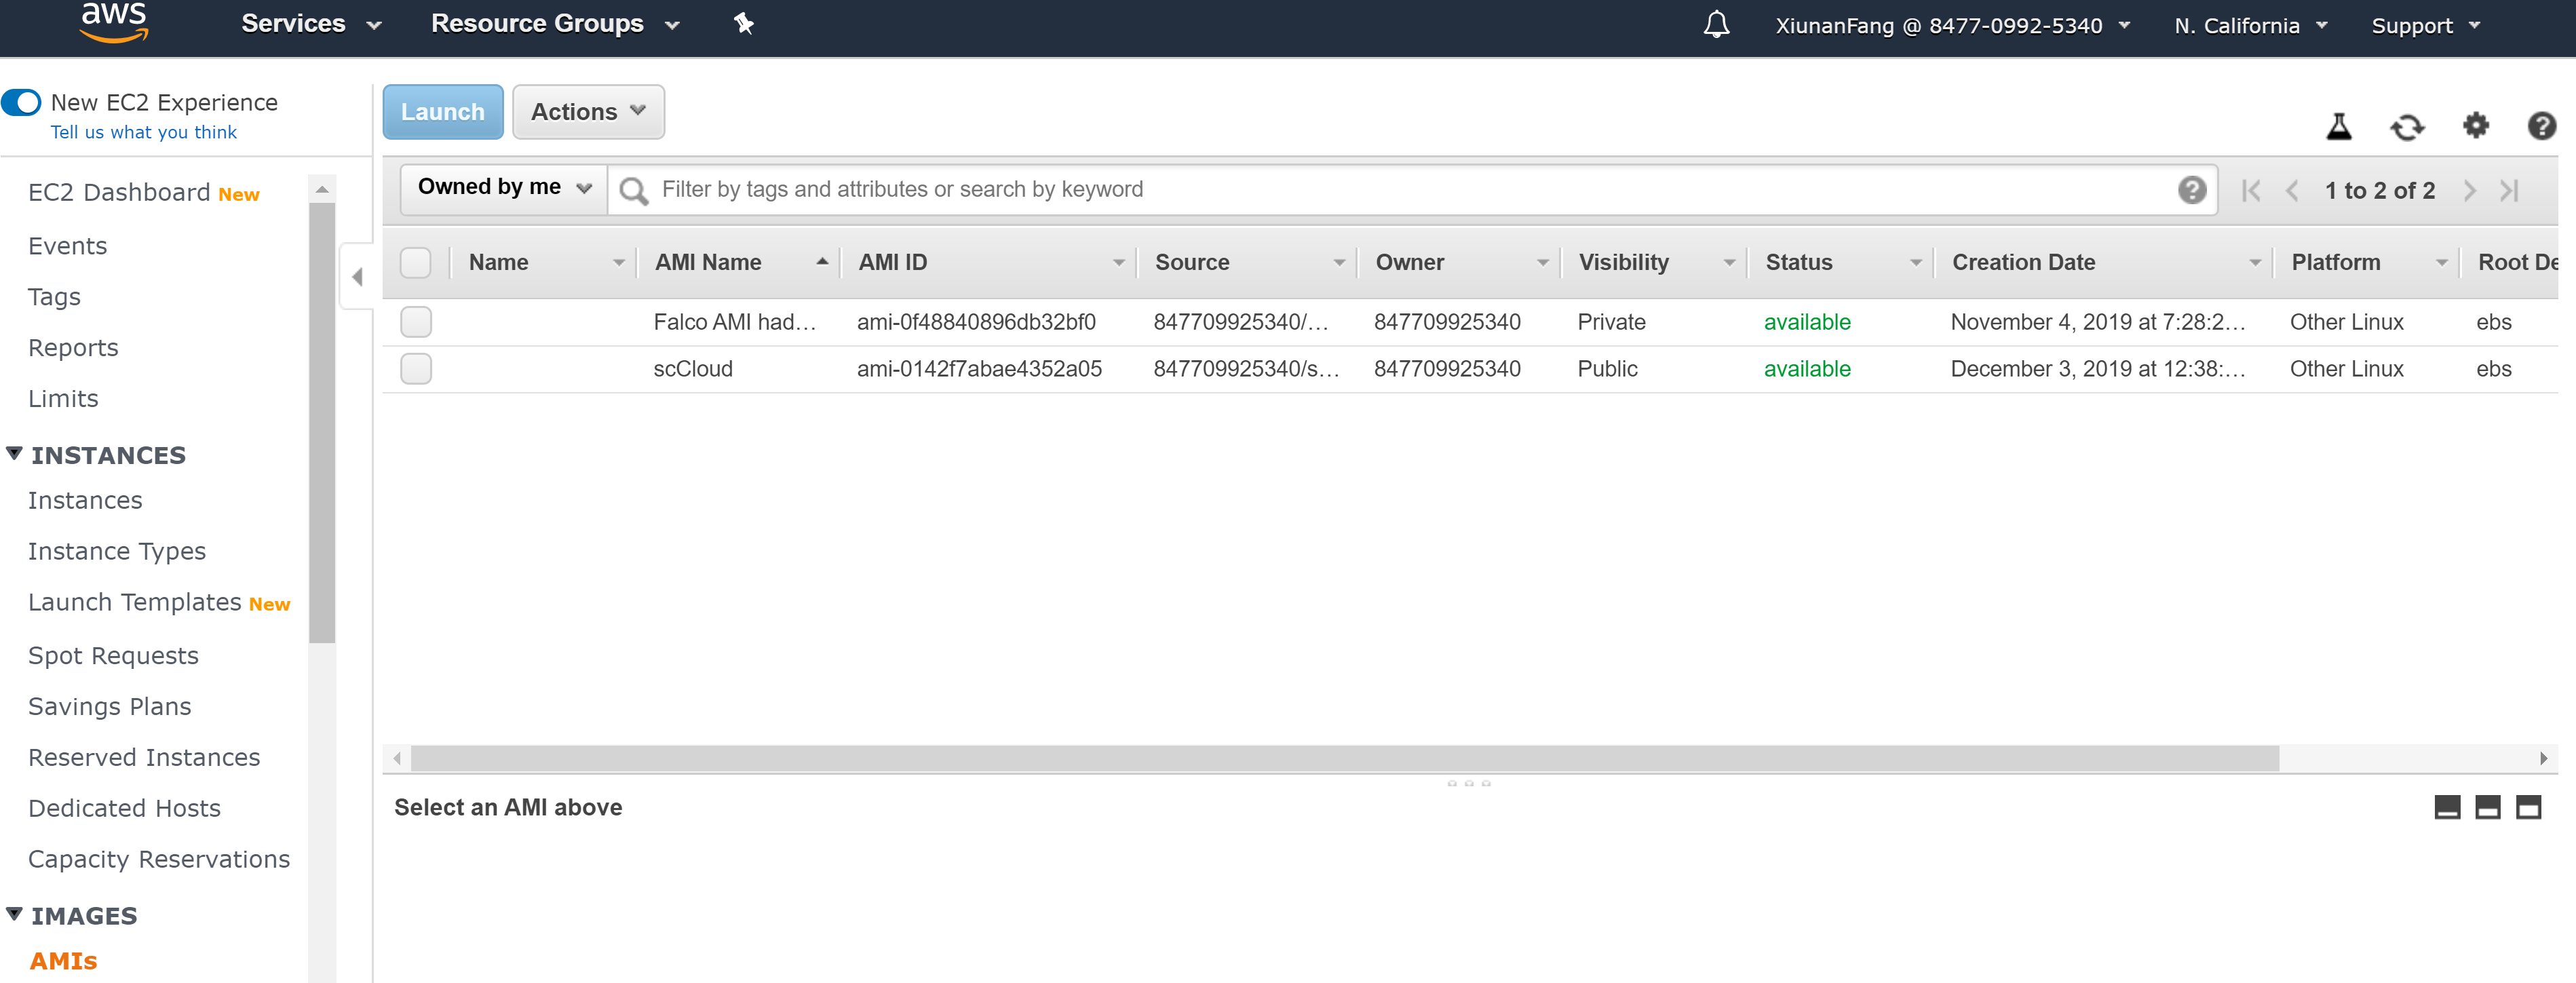
\includegraphics{falcoimage.PNG}

\hypertarget{run-the-tutorial}{%
\chapter{Run the tutorial}\label{run-the-tutorial}}

Change to Falco home directory.

\begin{verbatim}
cd $Faclco
\end{verbatim}

\hypertarget{give-values-for-s3-bucket-and-user-name}{%
\section{Give values for S3 bucket and User Name}\label{give-values-for-s3-bucket-and-user-name}}

The tutorial files have a number of locations that have a placeholder called username and yourbucket. Change these placeholders to your values. In a bash shell, from the \emph{Falco} home directory, edit and submit the following command:{[}❗️{]}

\begin{verbatim}
# preplace the bracketed sections with your details
sed -i.bak 's/username/[YOUR USER NAME]/g ; s/yourbucket/[YOUR BUCKET NAME]/g' tutorial/*.config
# EXAMPLE ONLY: if your user name if "fred" and your AWS bucket is "falco-test", then you would use the following command
#sed -i.bak 's/username/fred/g ; s/yourbucket/falco-test/g' tutorial/*.config
\end{verbatim}

\begin{verbatim}
sed -i.bak.reg 's/us-west-2/[YOUR REGION]/g' tutorial/*.config
# change [YOUR REGION] to the name of your region
# EXAMPLE (if your region is us-west-1): sed -i.bak.reg 's/us-west-2/us-west-1/g' tutorial/*.config
\end{verbatim}

The original .config files in the tutorial directory will now have the file extension .config.bak should you wish to restore the original files.

❗First open the file tutorial/emr\_cluster.config.

\begin{verbatim}
vi tutorial/emr_cluster.config
\end{verbatim}

Change the release\_label to the latest version:

\begin{verbatim}
release_label = emr-5.27.0
\end{verbatim}

Change the bootstrap\_scripts to only copy\_reference.sh:

\begin{verbatim}
bootstrap_scripts = copy_reference.sh
\end{verbatim}

Adding the line in the below:

\begin{verbatim}
# If custom AMI ID is specified, it is recommended to remove install_software.sh from thr bootstrap scripts as the custom AMI should already have these installed.
custom_ami_id = ami-0f48840896db32bf0
\end{verbatim}

and check that {[}EMR\_nodes{]} section is similar to the following:

\begin{verbatim}
[EMR_nodes]
key_name = yourkey
service_role = EMR_DefaultRole
instance_profile = EMR_EC2_DefaultRole
master_instance_type = m5.4xlarge
master_instance_count = 1
core_instance_type = m5.4xlarge
core_instance_count = 2
core_instance_spot = True
core_instance_bid_price = 1
\end{verbatim}

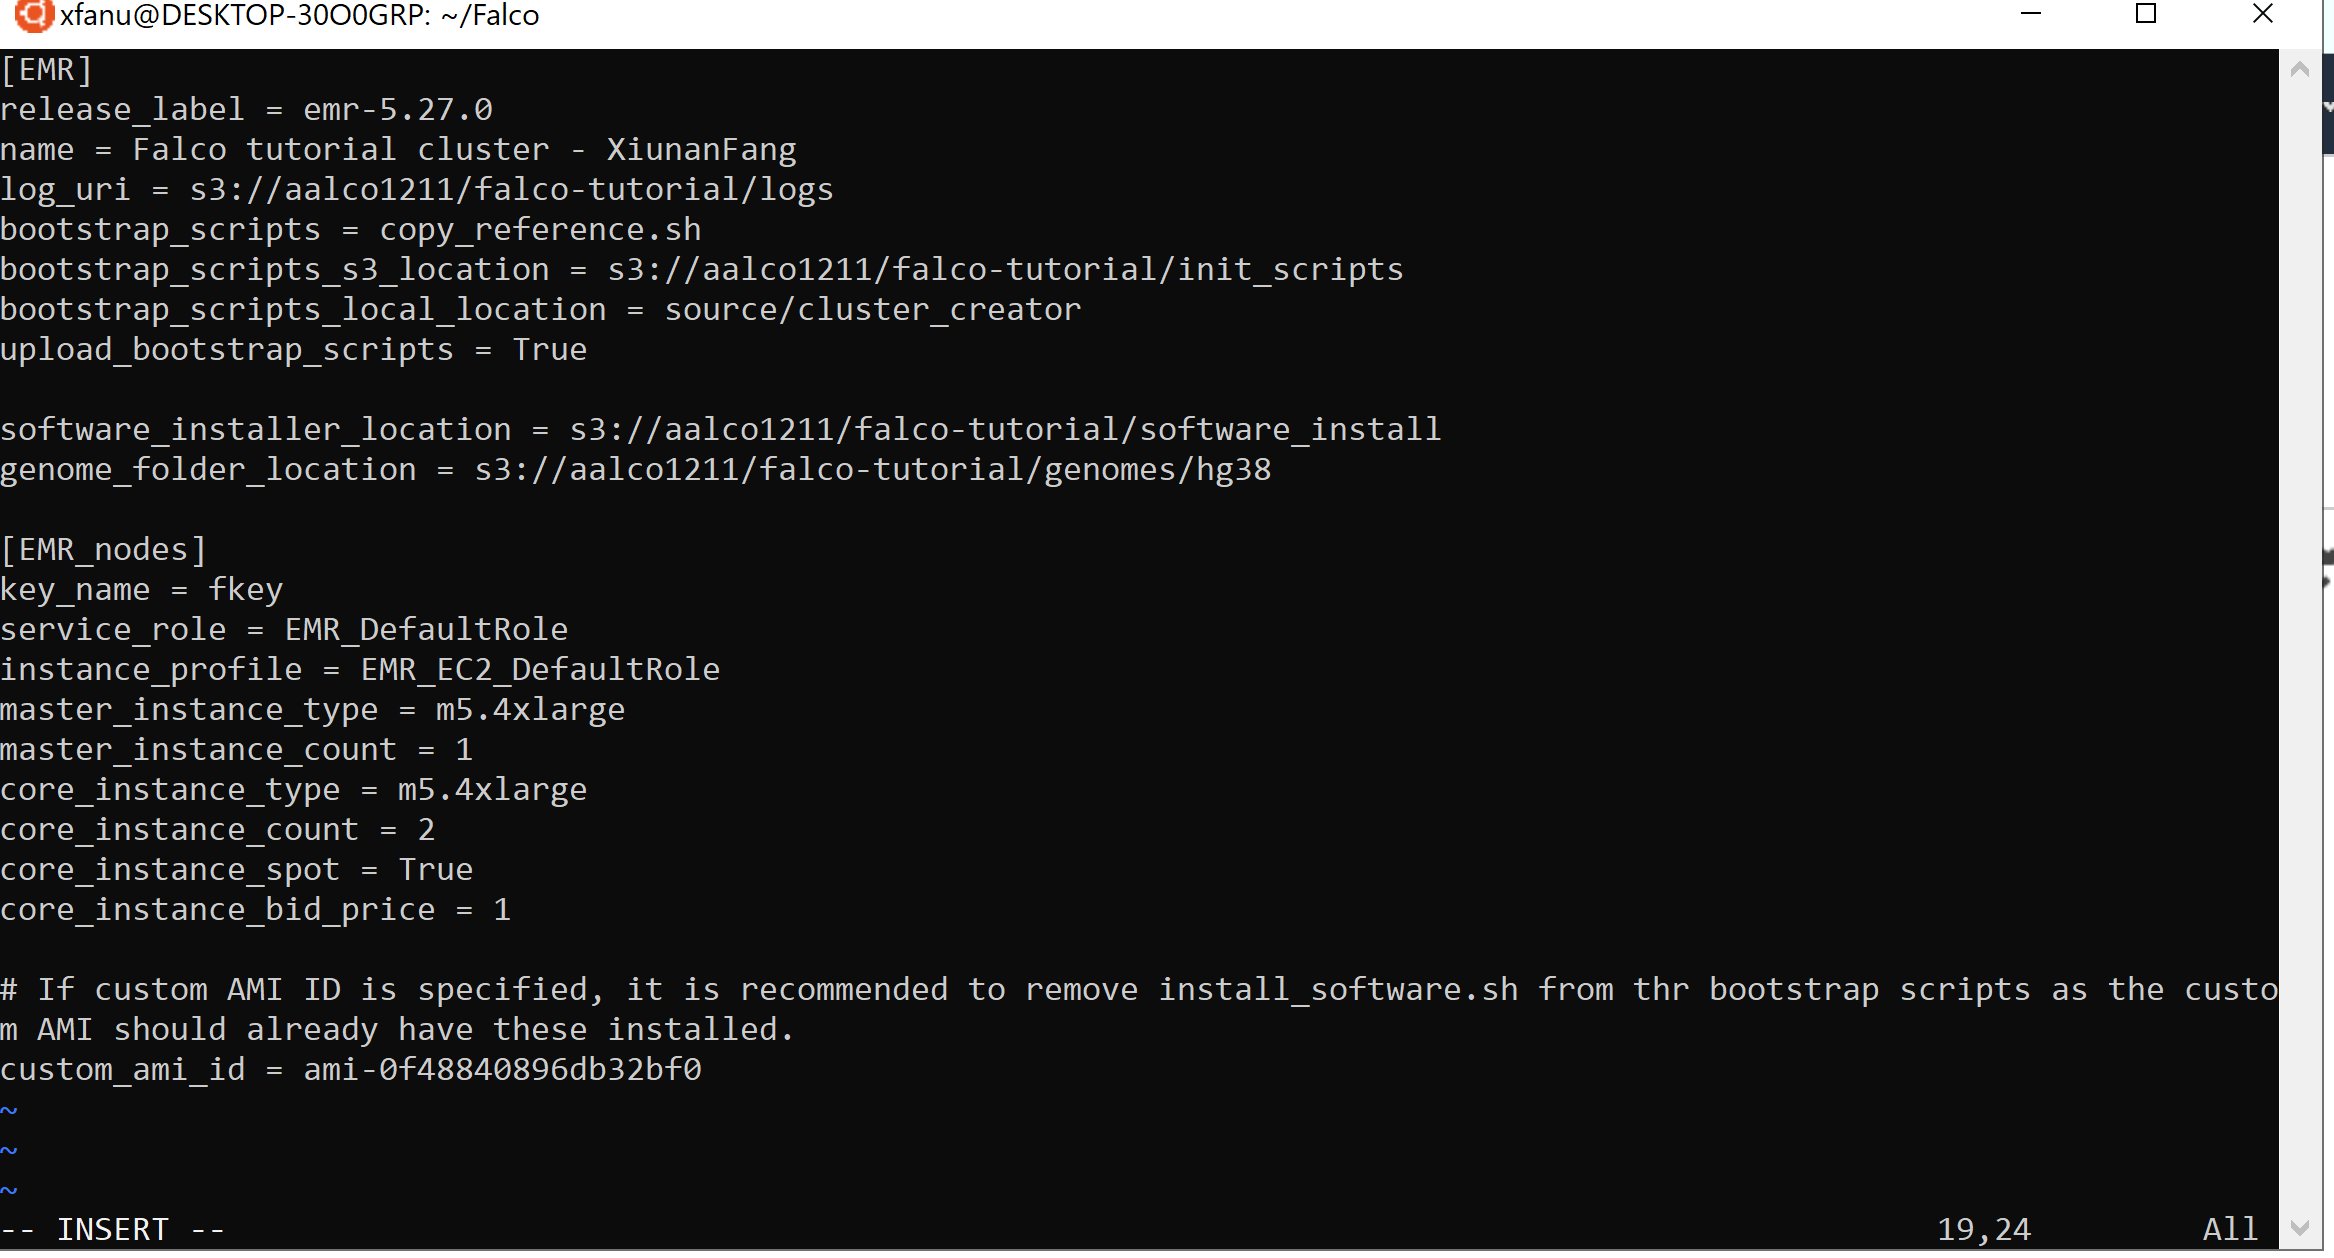
\includegraphics{emr_config.PNG}
The \texttt{{[}EMR\_nodes{]}} section contains a line that starts with \texttt{key\_name\ =}. The computing resources created by the AWS EMR framework uses public--key cryptography to encrypt and decrypt login information. You need to supply your key name here. For example, if your encryption key file is \texttt{my-key-name.pem}, the corresponding line in the configuration file should read \texttt{key\_name\ =\ my-key-name}. {[}❗️{]}Go ahead and edit this entry - enter your key name.{[}🔴{]}{[} Also be aware of the charges that you may incur from AWS for the creation of this cluster. The master instance will be an on-demand type, whilst the two core instances are spot instance types. It is estimated the cost of the cluster for this tutorial, if terminated within 1 hour, will be less than \$5 USD. This cost is based on the AWS region us-west-2 - US West (Oregon).

\hypertarget{launch-the-aws-emr-cluster}{%
\section{Launch the AWS EMR cluster}\label{launch-the-aws-emr-cluster}}

When ready, in the home directory of the \emph{Falco} code, issue the following command to start the cluster: {[}❗️{]}

\begin{verbatim}
python3 launch_cluster.py --config tutorial/emr_cluster.config
\end{verbatim}

When the command is processed, the user will receive a response, of the form:

\begin{verbatim}
Cluster has been launched with ID j-1FDPU9CHN79W9
\end{verbatim}

Make a note of your cluster ID for future reference.

\hypertarget{monitor-the-emr-cluster}{%
\section{Monitor the EMR Cluster}\label{monitor-the-emr-cluster}}

{[}❗️{]} Monitor the status of the EMR cluster via the AWS EMR console. When the status of your cluster is Ready, you may proceed with the steps required for completing the analysis.

Click on your cluster to obtain more information about your cluster.

{[}🔴{]} Since the nodes that are launched as part of this cluster use AWS spot instance types, it is possible that the market price for the instances exceeds the bid price. If this is the case, then the cluster will not start until the market price falls below the bid price. You can monitor the market price for the spot instances via the AWS EC2 Mangement Console. You can decide if you want to terminate your EMR cluster and either try again later, or modify the bid price in the file \texttt{tutorial/emr\_cluster.config}.

\hypertarget{upload-the-manifest-file}{%
\section{Upload the Manifest file}\label{upload-the-manifest-file}}

Falco requires a manifest file to list the FASTQ filenames representing the data input. The required format is a tab delimited text file. This file has been provided for this tutorial and is located at \texttt{tutorial/data.manifest}. Upload the manifest file to your AWS S3 bucket: {[}❗️{]}

\begin{verbatim}
# issue this command from the Falco home directory
aws s3 cp tutorial/data.manifest s3://[YOUR BUCKET]/falco-tutorial/data.manifest
# replace [YOUR BUCKET] with the name of your bucket
\end{verbatim}

{[}🔴{]}The following three instructions that launch jobs can be issued one after the other - without waiting for the previous job to finish. The EMR framework will launch jobs in order, and only after the previous job has completed.

\hypertarget{launch-the-split-job}{%
\section{Launch the Split job}\label{launch-the-split-job}}

The split job takes the original data and splits it into smaller sized files for more efficient processing by Falco. The original input data stored on AWS S3 will not be removed. The modified data will be stored in a new AWS S3 location as specified in the configuration file \texttt{tutorial/split\_job.config}. Type the following command at a command prompt in the Falco home directory:{[}❗️{]}

\begin{verbatim}
python3 submit_split_job.py --config tutorial/split_job.config
\end{verbatim}

\hypertarget{launch-the-pre-processing-job}{%
\section{Launch the Pre-processing job}\label{launch-the-pre-processing-job}}

In Falco, the pre-processing step is optional. However, for this tutorial, an example pre-processing script is provided, and this step is compulsory to complete the tutorial as configured.

First examine the configuration file \texttt{tutorial/preprocessing\_job.config}. The config file specifies which bash scripts are used for the pre-processing. You may wish to also examine these scripts to see how the pre-processing works in this case. Type the following at a command prompt from the Falco home directory: {[}❗️{]}

\begin{verbatim}
python3 submit_preprocessing_job.py --config tutorial/preprocessing_job.config
\end{verbatim}

\hypertarget{launch-the-analysis-job}{%
\section{Launch the Analysis job}\label{launch-the-analysis-job}}

This is the main analysis job that processes the pre-processed data to determine the counts of features. The output be two .csv files: the actual counts of features, and a separate file detailing quality assurance statistics relating to these counts.

The configuration file \texttt{tutorial/analysis\_job.config} contains the settings for the analysis job with STAR as the aligner and featureCount for quantification - including any extra parameters for the tools used. The configuration file also specifies the AWS S3 location for the final output .csv files. Enter the following at a command prompt from the Falco home directory: {[}❗️{]}

\begin{verbatim}
python3 submit_analysis_job.py --config tutorial/analysis_job.config
\end{verbatim}

{[}🔴{]} To change the alignment and/or quantification tool used in the analysis job, simply modify the \texttt{aligner\_tool} and \texttt{counter\_tool} option in the analysis configuration file (\texttt{analysis\_job.config}).

\hypertarget{monitor-steps}{%
\section{Monitor Steps}\label{monitor-steps}}

Note that, as long as the above three steps (split, preprocess, and analysis) are entered in that order, the steps may be entered one after the other - without having to wait until the previous step finishes. The EMR framework ensures that a step does not start until the previously queued step has completed.

{[}❗️{]} Monitor the status of each step using the AWS EMR console - in the Step section.

\hypertarget{monitor-s3-files}{%
\section{Monitor S3 files}\label{monitor-s3-files}}

Use the AWS S3 Console to monitor files in your S3 bucket.

\hypertarget{download-results-and-terminate-cluster}{%
\section{Download results and Terminate Cluster}\label{download-results-and-terminate-cluster}}

To download a file from AWS S3 to your current directory, edit the following command with your details and execute at a shell command line: {[}❗️{]}

\begin{verbatim}
aws s3 cp s3://[YOUR BUCKET]/falco-tutorial/[YOUR USER NAME]/analysis/samples_expression.csv .
# you can also list all the AWS S3 files that begin with a particular prefix:
#aws s3 ls s3://[YOUR BUCKET]/falco-tutorial/[YOUR USER NAME]/analysis/
\end{verbatim}

Alternatively, you could see a listing of the results via the AWS S3 Console by navigating to your bucket and output location.

\textbf{{[}🔴{]}As AWS charges by the hour for usage of its services, the user should terminate their cluster when finished. This is done by selecting your cluster on the AWS EMR console \emph{Cluster List}, and clicking the \emph{Terminate} button.}

\backmatter
  \bibliography{book.bib,packages.bib}

\end{document}
